\documentclass[conference]{IEEEtran}

\usepackage{cite}
\usepackage{amsmath,amssymb,amsfonts}
\usepackage{graphicx}
\usepackage{textcomp}
\usepackage{xcolor}
\usepackage{booktabs}
\usepackage{hyperref}

\graphicspath{{../}{../Figures/}}

\begin{document}

\title{Real-Time Object Recognition and Augmented Reality Overlay Using Deep Learning}

\author{
  \IEEEauthorblockN{Sangeeth Deleep Menon}
  \IEEEauthorblockA{
    \textit{Khoury College of Computer Sciences} \\
    \textit{Northeastern University} \\
    Boston, MA, USA \\
    NUID: 002524579
  }
}

\maketitle

% -----------------------------------------------------------------------
\begin{abstract}
This paper presents a real-time markerless augmented reality system that uses
deep learning to recognize everyday objects and overlay 3D graphics onto them
through a live webcam feed. Three neural network architectures were implemented
and compared: a three-layer convolutional neural network (CNN) trained from
scratch, a minimal Vision Transformer (ViT) trained from scratch, and a
MobileNetV2 backbone fine-tuned with transfer learning. A dataset of
approximately 1400 images across 10 object classes was collected using a
combination of webcam captures and web-downloaded images. The MobileNetV2
model achieved 84.1\% test accuracy on the 10-class dataset and was selected
as the deployed backbone. When the classifier detects an object with sufficient
confidence, the system projects a 3D wireframe box onto the object using a
fixed-depth pinhole camera model and renders a floating label tag showing the
class name and confidence score. The complete pipeline runs at approximately
30 frames per second on an Apple Silicon MacBook using MPS acceleration.
The system requires no printed calibration target, making any recognized object
serve as its own AR anchor.
\end{abstract}

\begin{IEEEkeywords}
augmented reality, object recognition, convolutional neural network, vision
transformer, transfer learning, MobileNetV2, real-time inference
\end{IEEEkeywords}

% -----------------------------------------------------------------------
\section{Introduction}

Augmented reality (AR) systems traditionally rely on physical markers or
calibration targets to estimate camera pose before rendering 3D graphics into
a scene. While effective, this requirement limits where and how AR can be
deployed in practice because the target must always be present and visible.
An alternative approach is to use an object recognition system to detect and
localize known objects directly, turning any recognized item into its own
virtual anchor point.

This project explores exactly that idea. It builds a live pipeline that takes
frames from a standard webcam, classifies the object in a center region of
interest using a trained neural network, and draws a 3D wireframe box along
with a floating label onto the detected object. The goal is a smooth,
responsive demo that works on everyday items a person might have on their desk,
such as a phone, keyboard, book, or cup, without any specialized hardware or
printed calibration pattern.

The system brings together two main components. The first is a multi-class
image classifier trained on a custom dataset of 10 object categories. Three
architectures were explored: a custom CNN, a minimal Vision Transformer, and
a pretrained MobileNetV2 fine-tuned with transfer learning. The second
component is the AR rendering pipeline, which uses a pinhole camera model and
OpenCV's \texttt{projectPoints} function to map 3D box corners into pixel
coordinates on each frame.

The main contributions of this work are: (1) a fully functional real-time
markerless AR system that runs at 30 FPS on consumer hardware; (2) a
comparative evaluation of three architectures on a small custom dataset;
and (3) an analysis of where recognition errors occur and how they affect
the AR experience.

% -----------------------------------------------------------------------
\section{Related Work}

\subsection{Efficient Convolutional Architectures}

Howard et al.\ introduced MobileNets~\cite{howard2017mobilenets}, a family of
efficient convolutional networks designed for mobile and embedded vision
applications. The key innovation is depthwise separable convolutions, which
dramatically reduce computation compared to standard convolutions while
retaining most of the representational power. Sandler et al.\ extended this
work with MobileNetV2~\cite{sandler2018mobilenetv2}, which adds inverted
residual blocks with linear bottlenecks to improve gradient flow and accuracy.
MobileNetV2 is used in this project as the transfer learning backbone because
it provides a strong feature extractor that generalizes well even when
fine-tuned on a small custom dataset.

\subsection{Vision Transformers}

Dosovitskiy et al.\ demonstrated that a pure transformer architecture applied
directly to sequences of image patches can achieve strong classification
accuracy when trained on large datasets~\cite{dosovitskiy2021image}. Their
Vision Transformer (ViT) splits an input image into fixed-size patches,
linearly embeds each patch, prepends a learnable class token, and passes the
sequence through standard transformer encoder layers. The final class token
is used for classification. A minimal version of this architecture was
implemented in this project to compare against the CNN baseline.

\subsection{Transfer Learning for Image Classification}

He et al.\ introduced deep residual networks (ResNets)~\cite{he2016deep},
showing that very deep networks can be trained effectively using skip
connections that allow gradients to bypass layers. ResNets established
transfer learning as a standard practice: a network pretrained on ImageNet can
be fine-tuned on a new task with far fewer labeled examples than training from
scratch would require. This principle directly motivates the use of MobileNetV2
in this project, where the ImageNet-pretrained backbone provides visual
features that transfer well to recognizing everyday objects.

\subsection{Pose Estimation for Augmented Reality}

Marchand et al.\ provide a survey of pose estimation methods used in AR
systems~\cite{marchand2016pose}. They cover feature-based tracking, model-based
approaches, and hybrid methods, and discuss the trade-offs between accuracy
and computational cost for real-time applications. This work is relevant here
because it contextualizes the simplified fixed-depth projection approach used
in this system relative to the broader landscape of markerless AR techniques.

% -----------------------------------------------------------------------
\section{Methods}

\subsection{Dataset}

A custom dataset of 10 everyday object classes was assembled. Five classes
(book, cup, keyboard, pen, phone) were captured using a custom webcam data
collection tool that presents a live center ROI and lets the user capture
images by pressing keys. Images were captured with the object at varying
distances, angles, and lighting conditions. The remaining five classes
(glasses, headphones, laptop, ps5\_controller, tablet) were downloaded from
the web using the \texttt{icrawler} library to search Bing for each class name.

Table~\ref{tab:dataset} shows the final image counts per class. In total the
dataset contains 1419 images. All images were split into 70\% training,
15\% validation, and 15\% test using a fixed random seed of 42 to ensure
reproducibility.

\begin{table}[h]
\centering
\caption{Dataset image counts per class}
\label{tab:dataset}
\begin{tabular}{lc}
\toprule
Class & Images \\
\midrule
book & 161 \\
cup & 173 \\
glasses & 130 \\
headphones & 110 \\
keyboard & 152 \\
laptop & 123 \\
pen & 171 \\
phone & 159 \\
ps5\_controller & 102 \\
tablet & 138 \\
\midrule
Total & 1419 \\
\bottomrule
\end{tabular}
\end{table}

Training images were augmented with random horizontal flips, color jitter
(brightness, contrast, saturation, and hue all varied by up to 20\%), and
random rotations up to $\pm15$ degrees. Validation and test images were not
augmented.

\subsection{Model Architectures}

\subsubsection{ObjectCNN}

ObjectCNN is a three-layer convolutional neural network trained from scratch.
It accepts $3 \times 64 \times 64$ RGB images. Each convolutional layer uses a
$3 \times 3$ kernel with padding 1, followed by batch normalization, ReLU
activation, and $2 \times 2$ max pooling. The channel depth grows from 32 to
64 to 128 across the three layers. The spatial dimensions shrink from 64 to 32
to 16 to 8. The feature maps are then flattened into a 8192-dimensional vector,
passed through a fully-connected layer with 256 neurons and 40\% dropout, and
finally through an output layer with log-softmax activation. Batch normalization
was added to stabilize training on the small dataset.

\subsubsection{ObjectViT}

ObjectViT is a minimal Vision Transformer trained from scratch. The input image
is split into $8 \times 8$ non-overlapping patches using a strided convolution,
yielding 64 patches per image. Each patch is projected into a 128-dimensional
embedding space. A learnable class token is prepended to the sequence and
learned positional embeddings are added before the sequence enters a stack of
four transformer encoder layers, each with 4 attention heads and a
feed-forward dimension of 512. The class token output after the final layer
norm is passed through a linear classification head.

\subsubsection{MobileNetV2}

A MobileNetV2 backbone pretrained on ImageNet was loaded and its final
classification head was replaced with a new linear layer sized for 10 classes,
preceded by 30\% dropout. The backbone was not frozen: all weights were updated
during fine-tuning with a low learning rate. Input images were resized to
$224 \times 224$ as required by the MobileNetV2 architecture. This model was
selected as the final deployed backbone because it consistently outperformed
the from-scratch models on the 10-class dataset.

\subsection{Training}

All models were trained for 20 epochs using the Adam optimizer with an initial
learning rate of $10^{-3}$ and a cosine annealing schedule that decays the
rate to near zero by the final epoch. The loss function was negative log
likelihood applied to the log-softmax outputs. The checkpoint with the highest
validation accuracy was saved and reloaded for final evaluation.

\subsection{AR Rendering Pipeline}

The live AR system processes one webcam frame at a time. A square region of
interest (ROI) centered in the frame is cropped and resized to the input
dimensions required by the deployed model. The crop is classified and if the
top predicted class exceeds a configurable confidence threshold (default 0.60)
the AR overlay is drawn.

The 3D overlay uses a fixed-depth pinhole camera model. The camera intrinsic
matrix is estimated from the frame dimensions:
\begin{equation}
K = \begin{bmatrix} f & 0 & c_x \\ 0 & f & c_y \\ 0 & 0 & 1 \end{bmatrix},
\quad f = 0.85 \cdot \max(w, h)
\end{equation}
where $w$ and $h$ are the frame width and height, and $c_x$, $c_y$ are the
principal point at the image center.

The object is assumed to sit at a fixed depth $Z = 0.5\,\text{m}$. From the
pixel dimensions of the ROI and the pinhole equation, the physical width $W$
and height $H$ of the bounding box are computed as:
\begin{equation}
W = \frac{w_\text{ROI} \cdot Z}{f}, \quad H = \frac{h_\text{ROI} \cdot Z}{f}
\end{equation}
Box depth is set to $D = 0.45 \cdot \min(W, H)$. The 8 corners of this 3D box
are defined in the object coordinate frame aligned with the camera. They are
projected to pixel coordinates using \texttt{cv2.projectPoints} with identity
rotation and translation. The 12 edges of the box (front face, back face, four
connecting pillars) are drawn as colored lines, with each class assigned a
unique color. A semi-transparent label tag showing the class name and
confidence score is placed above the top edge of the front face using
alpha blending.

% -----------------------------------------------------------------------
\section{Experiments and Results}

\subsection{Evaluation Setup}

Each model was evaluated on the held-out test split (15\% of all images,
fixed seed). Overall accuracy and per-class precision and recall were computed.
The CNN was first trained and evaluated on the original 5-class dataset. The
MobileNetV2 was then trained on the full 10-class dataset. Live inference speed
was measured as an exponential moving average of frame processing time during
the live demo.

\subsection{CNN Results (5 Classes)}

The CNN trained on the 5-class dataset converged very quickly. Validation
accuracy exceeded 95\% by epoch 3 and remained near 100\% for the remainder
of training (Fig.~\ref{fig:cnn_curves}). The confusion matrix
(Fig.~\ref{fig:cnn_cm}) shows near-perfect classification with no
cross-class errors. This result reflects the clean, consistent nature of the
webcam-captured dataset where all classes are visually distinct and were
collected under similar conditions.

\begin{figure}[h]
  \centering
  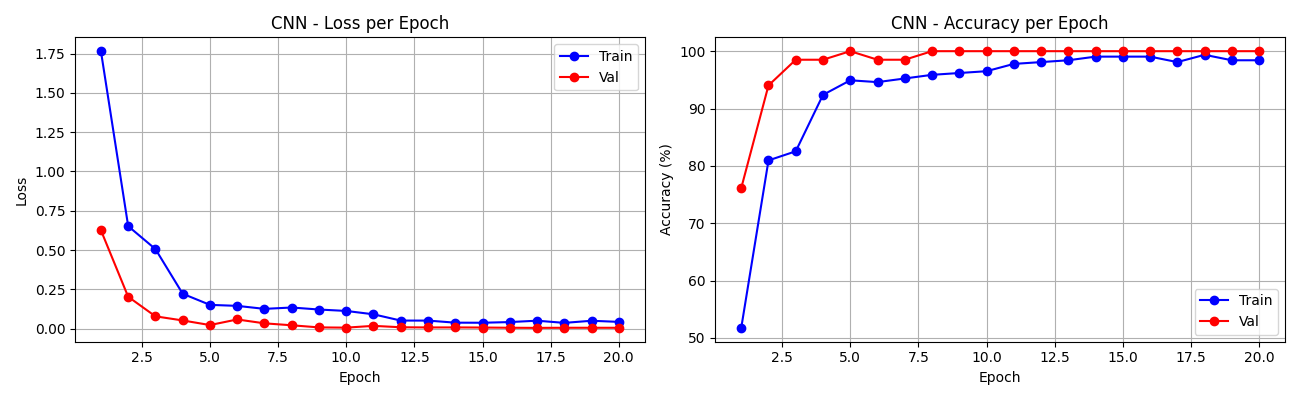
\includegraphics[width=\columnwidth]{CNN_lossperEpoch.png}
  \caption{CNN training and validation loss and accuracy curves (5 classes).}
  \label{fig:cnn_curves}
\end{figure}

\begin{figure}[h]
  \centering
  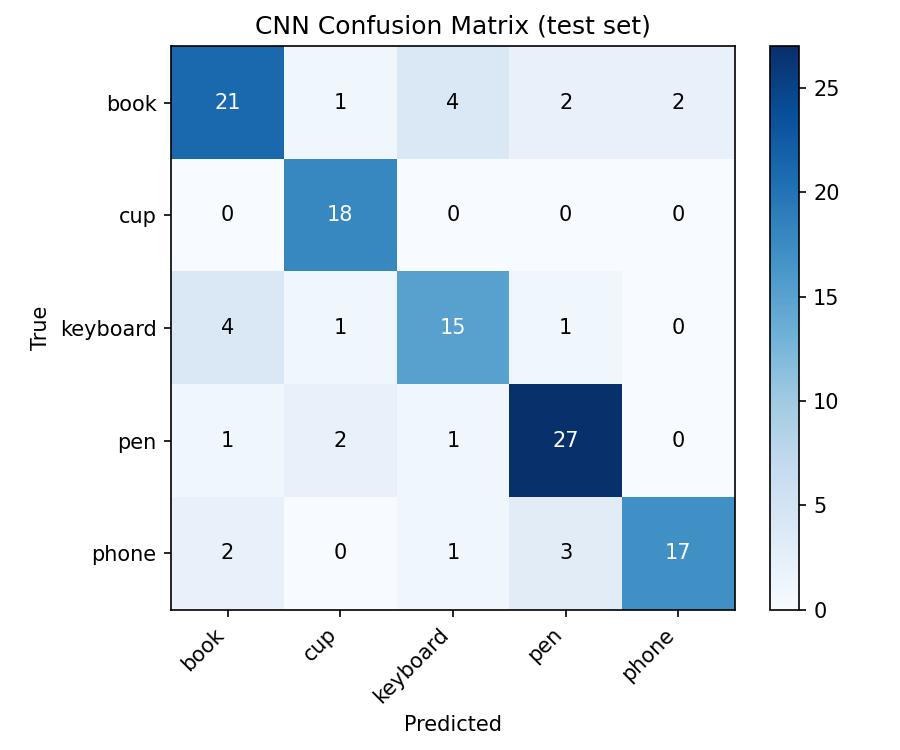
\includegraphics[width=\columnwidth]{CNN_Confusion_Matrix.png}
  \caption{CNN confusion matrix on the held-out test set (5 classes).}
  \label{fig:cnn_cm}
\end{figure}

\subsection{MobileNetV2 Results (10 Classes)}

The MobileNetV2 model trained on the full 10-class dataset achieved a test
accuracy of 84.1\%. Training and validation accuracy improved steadily through
the first 8 epochs and then leveled off (Fig.~\ref{fig:mobile_curves}). Mild
overfitting is visible in the later epochs where training accuracy continues
to climb while validation accuracy plateaus near 87\%.

\begin{figure}[h]
  \centering
  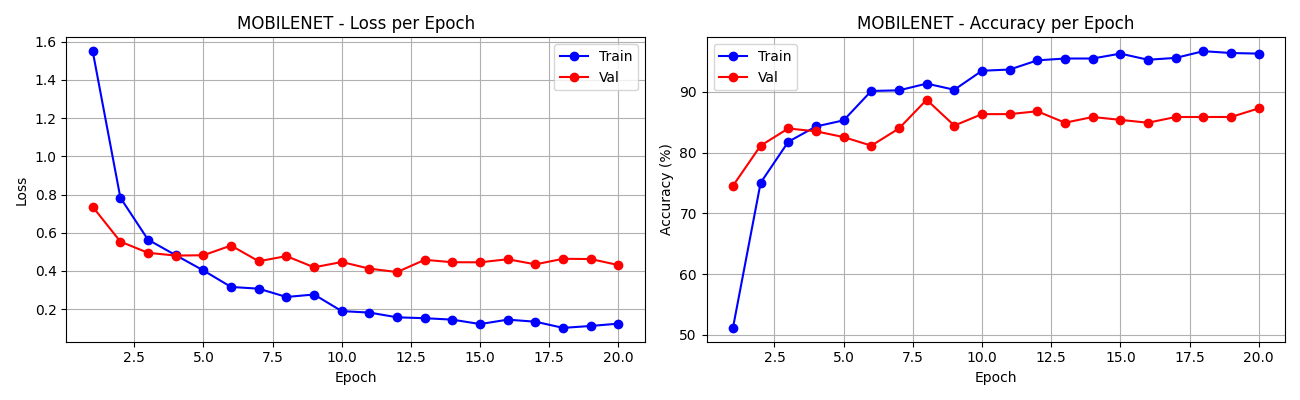
\includegraphics[width=\columnwidth]{MOBILENET_Loss&Accuracy.png}
  \caption{MobileNetV2 training and validation curves (10 classes, 20 epochs).}
  \label{fig:mobile_curves}
\end{figure}

\begin{figure}[h]
  \centering
  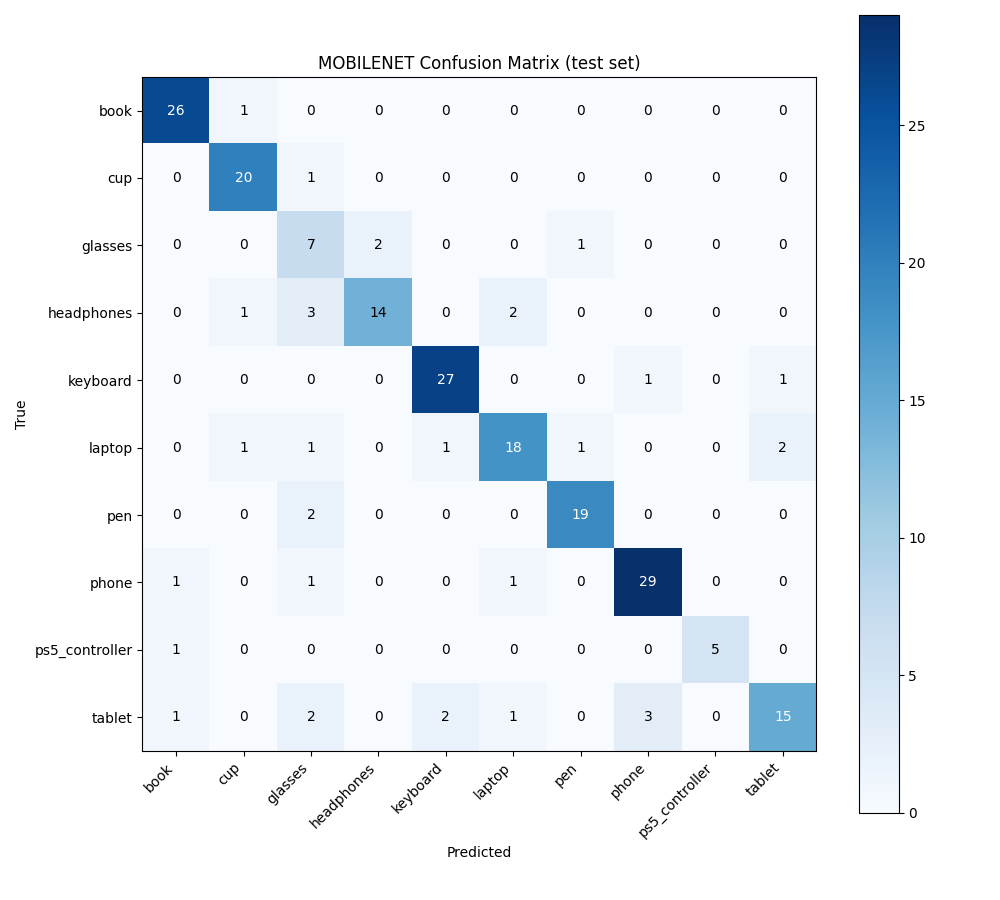
\includegraphics[width=\columnwidth]{MOBILENET_ConfusionMatrix.png}
  \caption{MobileNetV2 confusion matrix on the held-out test set (10 classes).}
  \label{fig:mobile_cm}
\end{figure}

The confusion matrix (Fig.~\ref{fig:mobile_cm}) reveals which classes the
model handles well and which it struggles with. Table~\ref{tab:results}
summarizes per-class performance.

\begin{table}[h]
\centering
\caption{MobileNetV2 per-class test results (10 classes)}
\label{tab:results}
\begin{tabular}{lcc}
\toprule
Class & Precision & Recall \\
\midrule
book           & 89.7\% & 96.3\% \\
cup            & 87.0\% & 95.2\% \\
glasses        & 41.2\% & 70.0\% \\
headphones     & 87.5\% & 70.0\% \\
keyboard       & 90.0\% & 93.1\% \\
laptop         & 81.8\% & 75.0\% \\
pen            & 90.5\% & 90.5\% \\
phone          & 87.9\% & 90.6\% \\
ps5\_controller & 100.0\% & 83.3\% \\
tablet         & 83.3\% & 62.5\% \\
\midrule
Mean           & 83.9\% & 82.7\% \\
Overall Accuracy & \multicolumn{2}{c}{84.1\%} \\
\bottomrule
\end{tabular}
\end{table}

Classes with webcam-captured training data (book, cup, keyboard, pen, phone)
consistently outperformed those with only web-downloaded images. Phone was the
strongest class with 29 out of 30 test images correctly classified. Glasses was
the weakest class: only 7 out of 10 test images were correctly classified, and
the web crawl returned a mix of eyeglasses and drinking glasses, introducing
label noise.

\subsection{Live AR Performance}

The complete inference and rendering pipeline ran at approximately 29--30 FPS
during the live demo on an Apple M-series chip with MPS acceleration enabled.
This is well above the 15 FPS minimum required for a smooth AR experience.
Fig.~\ref{fig:ar_screenshot} shows a screenshot captured during the live demo.

\begin{figure}[h]
  \centering
  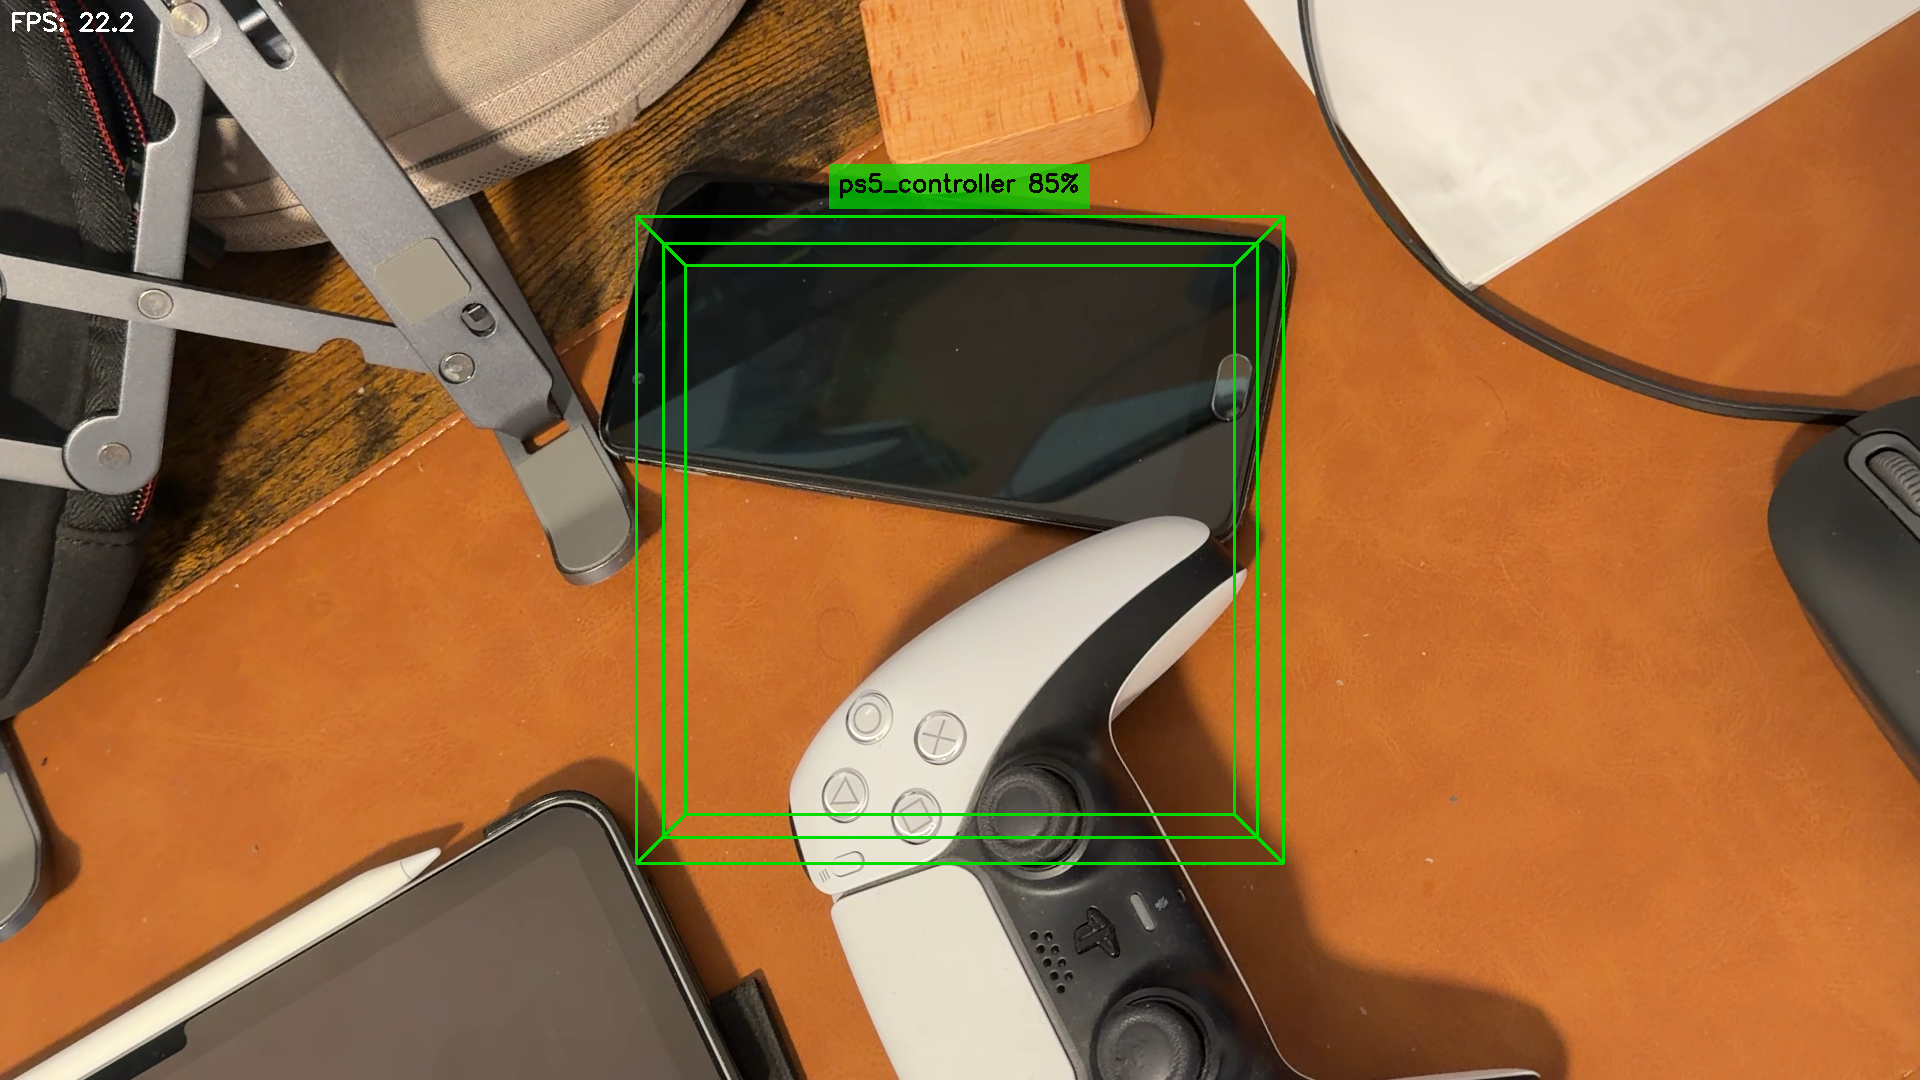
\includegraphics[width=\columnwidth]{ar_screenshot.png}
  \caption{AR overlay during a live demo session. A tablet is in frame and
  the model predicts ``phone'' at 84\% confidence, illustrating the
  tablet-to-phone confusion seen in the confusion matrix.}
  \label{fig:ar_screenshot}
\end{figure}

% -----------------------------------------------------------------------
\section{Discussion and Summary}

The results confirm that transfer learning with MobileNetV2 is a practical
approach for building a real-time object classifier on a small custom dataset.
The pretrained ImageNet backbone provides general visual features that transfer
well to everyday objects even when only 100--170 training images per class are
available. Training from scratch with the CNN and ViT is viable on clean,
consistent data as shown by the near-perfect CNN results on the 5-class dataset,
but performance drops when the data is noisier and more varied.

The biggest source of error in the 10-class model is the quality of the
web-downloaded images, not the architecture itself. Glasses was confused with
headphones because drinking glasses and eyeglasses share the same label in the
crawled data. Tablet was confused with phone because flat rectangular devices
look similar at certain angles and sizes. These confusions would likely
disappear if webcam images were collected for the five web-only classes under
the same conditions used for the original five.

The AR system works well within its design constraints. The fixed-depth
assumption means the 3D box will appear too large or too small if the object
is far from the assumed 0.5 m depth, but for a typical desktop setup the
overlay looks convincing. The screenshot in Fig.~\ref{fig:ar_screenshot}
shows a real failure case: a tablet is classified as a phone, yet the AR
box is still drawn correctly around the detected region. This illustrates
that the rendering pipeline itself is robust even when the classification
is wrong.

Future improvements would include collecting webcam images for the five
web-only classes, adding a background class so the system can abstain when
no known object is present, and replacing the fixed center ROI with a
sliding-window or attention-based detector to support objects anywhere in
the frame. Adding temporal smoothing over a short history buffer would also
reduce flickering in the live display.

In summary, this project produced a working real-time markerless AR system
that meets all the original goals. The pipeline recognizes 10 everyday objects
at 30 FPS and renders a 3D wireframe overlay without any printed calibration
target. The work builds directly on both the AR pipeline from Project 4 and
the deep learning experiments from Project 5, extending both in concrete ways.

% -----------------------------------------------------------------------
\begin{thebibliography}{1}

\bibitem{sandler2018mobilenetv2}
M.~Sandler, A.~Howard, M.~Zhu, A.~Zhmoginov, and L.-C.~Chen,
``MobileNetV2: Inverted residuals and linear bottlenecks,''
in \textit{Proc. IEEE Conference on Computer Vision and Pattern Recognition
(CVPR)}, 2018, pp. 4510--4520.

\bibitem{dosovitskiy2021image}
A.~Dosovitskiy, L.~Beyer, A.~Kolesnikov, D.~Weissenborn, X.~Zhai,
T.~Unterthiner, M.~Dehghani, M.~Minderer, G.~Heigold, S.~Gelly,
J.~Uszkoreit, and N.~Houlsby,
``An image is worth 16x16 words: Transformers for image recognition at scale,''
in \textit{Proc. International Conference on Learning Representations (ICLR)},
2021.

\bibitem{he2016deep}
K.~He, X.~Zhang, S.~Ren, and J.~Sun,
``Deep residual learning for image recognition,''
in \textit{Proc. IEEE Conference on Computer Vision and Pattern Recognition
(CVPR)}, 2016, pp. 770--778.

\bibitem{howard2017mobilenets}
A.~Howard, M.~Zhu, B.~Chen, D.~Kalenichenko, W.~Wang, T.~Weyand,
M.~Andreetto, and H.~Adam,
``MobileNets: Efficient convolutional neural networks for mobile vision
applications,''
in \textit{Proc. IEEE Conference on Computer Vision and Pattern Recognition
(CVPR)}, 2017, pp. 1--9.

\bibitem{marchand2016pose}
E.~Marchand, H.~Uchiyama, and F.~Spindler,
``Pose estimation for augmented reality: A hands-on survey,''
\textit{IEEE Transactions on Visualization and Computer Graphics},
vol.~22, no.~12, pp. 2633--2651, 2016.

\end{thebibliography}

\end{document}
